% FILE: main.tex  Version 2.1
% AUTHOR:
% Universit�t Duisburg-Essen, Standort Duisburg
% AG Prof. Dr. G�nter T�rner
% Verena Gondek, Andy Braune, Henning Kerstan
% Fachbereich Mathematik
% Lotharstr. 65., 47057 Duisburg
% entstanden im Rahmen des DFG-Projektes DissOnlineTutor
% in Zusammenarbeit mit der
% Humboldt-Universitaet zu Berlin
% AG Elektronisches Publizieren
% Joanna Rycko
% und der
% DNB - Deutsche Nationalbibliothek

\chapter{Discourse-Aware Sentiment Analysis}

Albeit coarse-grained seniment methods do a fairly good job at
classifying the overall polarity of a message, and DL-based approaches
also try their best to incorporate the compositional principle into
that prediction, a crucial limitation of all these systems is that
they overlook the structural nature of their input by either
considering it as a single whole (\eg{} bag-of-features approaches) or
analyzing it as a monotone sequence of equally important elements
(\eg{} recurrent neural methods).  Unfortunately, both of these
solutions completely ignore the hierarchical nature of language
\cite{Saussure:90,Hjelmslev:70}, in which morphemes are put together
to form words, words are united together into sentences, and multiple
sentences constitute a discourse.  Moreover, apart from this inherent
system hierarchy, even units of the same language level might play a
different role and be of varying importance while joined
syntagmatically: \eg{} in words, the root morpheme typically possesses
more lexical information than the affixes; in sentences, the syntactic
head usually dominates all its dependents.  The same kind of structure
can also be obsered in discourse, where one of the sentences might
express the core idea of the whole text.

Exactly the lack of the discourse information was the main reason for
the misclassifications of the systems of \citet{Severyn:15},
\citet{Baziotis:17}, and our own LBA method in Examples
\ref{snt:cgsa:exmp:severyn-error}, \ref{snt:cgsa:exmp:baziotis-error},
and \ref{snt:cgsa:exmp:lba-error} of the previous chapter.  Since none
of these approaches explicitly took the discourse structure into
account (in the best case, the inference simply proceeded from the
level of words directly to the level of a message), we decided to
check whether making the last of these solutions (the LBA classifier)
aware of the discourse phenomena would improve its results.  But,
before we begin with our experiments, we should first give a short
introduction to the most popular approaches to discourse analysis in
the literature and justify our choice of one of them.  Afterwards, in
Section~\ref{sec:dasa:data}, we will describe the way of inferring and
adding discourse information to the PotTS and SB10k data.  Then, in
Section~\ref{sec:dasa:data}, we will present a concise survey of the
existing discourse-aware sentiment analysis (DASA) methods and
evaluate their results on the two aforementioned corpora.  After
analyzing the effects of different common factors (such as various
subsets of discourse relations that might be used in a discourse-aware
sentiment system), we will summarize our findings in the last section
of this part.

\section{Discourse Analysis}\label{sec:dasa:theory}

Since the main focus of this chapter will be on \emph{discourse
  analysis}, we should first clarify what discourse analysis actually
means and which common ways there are to represent and analyze
discourse automatically.

In a nutshell, discourse analysis is an area of research in
linguistics and natural language processing which explores and
analyzes language phenomena beyond the sentence level \cite{Stede:11}.
Although the scope of this research can be quite large (ranging from
the use of pronouns in a sentence to the logical composition of a
document), in our experiments we will primarily concentrate on the
coherence structure of the text, \ie{} its segmentation into
\emph{elementary discourse units} (EDUs) and induction of
(hierarchical) \emph{coherence relations} between these EDUs.

Admittedly, the idea of decomposing the discourse into smaller
meaningful pieces and inferring semantic links between those parts
dates back to the very origins of general linguistics
\cite{Aristotle:10} and, in particular, its structuralism branch
\cite{Saussure:90}.  However, an especially big surge of interest in
this field happened in the 1970-s with the groundbreaking works of
\citet{vanDijk:72} and \citet{vanDijk:83}, who introduced the notion
of local and global coherence, defining the former as a set of ``rules
and conditions for the well-formed concatenation of pairs of sentences
in a linearly ordered sequence'' and specifying the latter as
contraints on the macro-structure of the narrative
\cite[see][]{Hoey:83}.  Similar ideas were also proposed
by~\citet{Longacre:79,Longacre:96}, who considered the paragraph as
another level of tagmemic grammar, which was composed of multiple
sentences according to a predefined set of compositional principles.
\todo{Replace ``finally''}{Finally,} \citet{Winter:77} presented an
extensive study of different lexical means, which could connect two
sentences, and also devised a taxonomy of semantic relattions based on
these observations.  All links in this taxonomy were divided into two
main groups: \textsc{Matching} and \textsc{Logical Sequence};
depending on whether a sentence was elaborating on the preceding
content of the text or rather adding new information to the narrative.

It is also not surprising that the increased interest of traditional
linguistics in text-level phenomena has also rapidly spurred the
attention of the broad NLP community to the discourse structure.
Among the first who affirmed the importance of discourse analysis for
automatic generation and understanding of texts was \citet{Hobbs:79},
who argued that semantic ties between sentences were the most
important component for building a coherent discourse, and the lexical
cohesion (\ie{} the use of coreferent and overlapping lexical items in
text) was an immediate corollary of these relations.  Similarly to
\citeauthor{Winter:77}, \citeauthor{Hobbs:79} also proposed a set of
possible inter-sentence relations, which, however, comprised only
three elements: \textsc{Elaboration}, \textsc{Parallel}, and
\textsc{Contrast}.  Although this taxonomy was obviously too small to
cover the whole variety of different semantic links that could exist
between sentences, it had laid the foundation of many successful
approaches to automatic discourse processing that appeared later.

\textbf{RST} One of the presumably best-known such approaches, called
\emph{Rhetorical Structure Theory} or \emph{RST}, was presented
by~\citet{Mann:88}.  Besides revising \citeauthor{Hobbs:79}' inventory
of discourse relations and expanding it to a set of 23 elements (by
including new items such as \textsc{Evidence}, \textsc{Elaboration},
\textsc{Circumstance}, etc.), the authors also introduced the
distinction between nucleus-satellite and multinuclear relations,
depending on whether two clauses connected by a semantic link were of
different importance to the content of the complete text
(nucleus-satellite) or represented equally significant,
interchangeable elements (multinuclear relations).  Following this
distinction, they formally defined each relation as a set of
constraints on the \emph{Nucleus} (N), \emph{Satellite} (S), \emph{the
  N+S combination}, and \emph{the effect} of the whole combination on
the reader (R).  An excerpt from the original description of the
\textsc{Evidence} link as defined by~\citet{Mann:88} is shown in
Example~\ref{dasa:exmp:rst-evidence}

\begin{example}[Definition of the \textsc{Evidence} Relation]\label{dasa:exmp:rst-evidence}
\textbf{Relation Name:} \textsc{Evidence}

\textbf{Constraints on N:} R might not believe N to a degree
satisfactory to W

\textbf{Constraints on S:} The reader believes S or will find it
credible

\textbf{Constraints on the N+S Combination:} R's comprehending S
increases R's belief of N

\textbf{Effect:} R's belief of N is increased

\textbf{Locus of the Effect:} N
\end{example}

\noindent However, the most important novelty of RST concerned not the
relations but the overall structure of the text, which, according to
the authors, had to be a (projective) tree, whose nodes were either
elementary discourse units or other subtrees, and edges were formed by
the semantic links holding between these parts.  A combination of a
nucleus and satellite node (or multiple nuclei in the case of a
multi-nuclear relation) in this tree formed an abstract node, which
essentially comprised the content of all its descendents, and could in
turn serve as a nucleus or satellite in further relations.  Thanks to
this structure, the root EDU of the top-most nucleus node\footnote{By
  root we mean the nucleus of the nucleus.} by definition represented
the central claim of the whole text, and satellite units that were
located closer to the top of the tree were supposed to have a larger
modification scope than their dependents.

You can see an example of an RST tree from the original Rhetorical
Structure Treebank \cite{Carlson:01a} in
Figure~\ref{dasa:fig:rst-tree}.  The top-most nucleus in this example
(\texttt{profit \ldots is estimated to have climbed between 11\% and
  14\%}) indeed expresses the main idea of the whole passage, while
other EDUs either specify the authorship of the message or provide
additional information on its claims, such as, for example, a
commentary of another expert.

\begin{figure*}[htbp!]
  {
  \centering
  \dirrel{}{
    \dirrel{Attribution}
           {\rstsegment{\refr{1}}}
           {}
           {\rstsegment{\refr{2}}}}
         {Interpretation-S}
         {\dirrel{Antithesis}
           {\rstsegment{\refr{3}}}
           {}
           {
             \dirrel{Attribution}
                    {\rstsegment{\refr{4}}}
                    {}
                    {
                      \dirrel{}
                             {
                               \dirrel{}{\rstsegment{\refr{5}}}{Comparison}{\rstsegment{\refr{6}}}
                             }
                             {Condition}
                             {\rstsegment{\refr{7}}}
                    }
           }
         }

         \begin{flushleft}
           \begin{rhetoricaltext}
             \unit[1]{Analysts said,}
             \unit[2]{profit for the dozen or so big drug makers, as a group, is estimated to have climbed between 11\% and 14\%.}
             \unit[3]{While that's not spectacular,}
             \unit[4]{Neil Sweig, an analyst with Prudential Bache, said}
             \unit[5]{that the rate of growth will ``look especially good}
             \unit[6]{as compared to other companies}
             \unit[7]{if the economy turns downward.''}
             \rstsource{\cite[WSJ-2341; ][]{Carlson:01a}}
           \end{rhetoricaltext}
         \end{flushleft}
         \caption[RST Tree Example]{Example of an RST-Tree}\label{dasa:fig:rst-tree}
}

\end{figure*}

Despite its immense popularity and practical utility \cite[see
][]{Marcu:98,Yoshida:14,Bhatia:15,Goyal:16}, RST has often been
criticized for the rigidness of the imposed tree structure
\cite{Wolf:05} and arbitrariness of the relation taxonomy
\cite{Nicholas:94,Miltsakaki:04}.  As a consequence of this criticism,
two alternative approaches to automatic discourse analysis have
entered the scene.

\textbf{PDTB} The first of these approaches---PDTB (named so after the
Penn Discourse Treebank \cite{Prasad:04})---has been developed by the
research group of the University of Pennsylvania
\cite{Miltsakaki:04,Miltsakaki:04a,Prasad:08}, and, at its core,
represents an \emph{underspecification of RST}, where, instead of
fully specifying the hierarchical structure of the text and trying to
come up with a comprehensive set of unambiguous discourse relations,
the author proceeded bottom-up, focusing on the grammatical and
lexical elements which could connect two sentences.  These elements
were typically either coordinating or subordinating conjunctions
(\eg{} \emph{and}, \emph{because}, \emph{since}, etc.) or discourse
adverbials (\eg{} \emph{however}, \emph{otherwise}, \emph{as a
  result}, etc.).  According to the original definition, each of these
connectives had to accept two sentence arguments: \textsc{Arg1} and
\textsc{Arg2}; and express a semantic \emph{sense} holding between
these predicates.  The choice of these senses was explicitly
restricted for each word: for example, the set of possible senses for
\emph{nonetheless} included \textsc{Comparison}, \textsc{Conjunction},
\textsc{Contra-Expectation}, and \textsc{Contrast}.

Apart from the explicitly mentioned connectives, \citet{Prasad:04}
also allowed for the situations where the connective was missing but
could be easily inferred from the context.  The authors denoted these
cases as \textsc{Implicit} discourse relations and asked the
annotators of the treebank to annotate the arguments of such relations
as well, but, in addition, also specify the connective word or phrase,
which, in their opinion, was omitted.

Finally, if there was neither an explicit nor an implicit connective,
\citet{Prasad:04} distinguished three different possibilities:
\begin{inparaenum}[(i)]
  \item either the coherence relation was expressed by an alternative
    lexical means which made the connective redundant
    (\textsc{AltLex}), or
  \item it was achieved by referring to the same entities in both
    sentences (\textsc{EntRel}), or
  \item there was no coherence relation at all (\textsc{NoRel});
\end{inparaenum}
and asked the experts to annotate such situations respectively with
different labels.  At last, in case of reported speech, PDTB also
provided a special \textsc{Attribution} tag for the text spans which
specified the authors of the statements.

Example~\ref{dasa:exmp:pdtb-analysis} shows the previous fragment of
the Wall Street Journal now annotated according to the PDTB scheme.
As we can see from the analysis, the PDTB approach is indeed more
flexible in comparison with RST as it allows the discourse units
(arguments) to overlap, be disjoint or even embedded into other
segments.  The assignment of sense relations is also more
straightforward and mainly determined by the connective that links the
arguments (\eg{} \emph{in fact}, \emph{while}, or \emph{if}).  At the
same time, the structure of this annotation is completely flat so that
we can neither infer which of the sentences plays the central role in
the text nor see the scope of modifying statements.

\begin{example}[Example of PDTB Analysis]\label{dasa:exmp:pdtb-analysis}
\fbox{Analysts said,} \argone[1]{profit for the dozen or so big drug
  makers, as a group, is estimated to have climbed between 11\% and
  14\%.}  \connective[1]{\textsc{implicit}$:=$in fact}
\argtwo[1]{\connective[2]{\textsc{explicit}$:=$While}
  \argtwo[2]{that's not spectacular}}, \fbox{Neil Sweig, an analyst
  with Prudential Bache, said} \argtwo[1]{\argone[2]{\argone[3]{that
      the rate of growth will ``look especially good as compared to
      other companies} \connective[3]{\textsc{explicit}:
      if}\argtwo[3]{the economy turns downward}}}.''
\end{example}

\textbf{SDRT} Another alternarive to RST---Segmented Discourse
Representation Theory or SDRT---was proposed by \citet{Lascarides:01}.
Although developed from a completely different angle of view (the
authors of SDRT mainly drew their inspiration from predicate logics,
dynamic semantics, and anaphora theory), SDRT shares many of its
features with the standard rhetorical structure, as it also assumes a
graph-like structure of the text, whose nodes are either elementary or
complex discourse units, and distinguishes between coordinating and
subordinating relations.  However, unlike RST, segmented discourse
representation explictly allows the text structure to be any graph,
not only tree (\ie{} a discourse node can have multiple parents and
also be connected via multiple links to the same vertex), provided
that it does not have crossing dependencies (right-frontier
constraint).  In this respect, SDRT can be viewed as a
\emph{structural relaxation of RST}.

We can also notice the relatedness of the two approaches by looking at
the SDRT analysis of the WSJ fragment in
Example~\ref{dasa:fig:sdrt-graph}.  Although the names of the
relations in the presented graph are completely different from those
used in RST, many of these relations have the same (or at least
similar) meaning as the respective links in the rhetorical structure:
for example, the \textsc{Source} relation in SDRT almost completely
corresponds to the \textsc{Attribution} edge in RST.  On the other
hand, SDRT's \textsc{Contrast} subsumes RST's \textsc{Contrast},
\textsc{Antithesis}, and \textsc{Comparison}, but, unlike the last two
nucleus-satellite links, represents a paratactic relationship between
the arguments.  These discrepancies between paratactic dependencies in
SDRT and their hypotactic equivalents in RST account for the lion's
share of the differences between the two discourse representations in
Examples~\ref{dasa:fig:rst-tree} and \ref{dasa:fig:sdrt-graph}.
Another dissimilarity stems from the different scopes of the
commentary \texttt{While that's not spectacular} assigned by SDRT and
RST: while the SDRT graph suggests that this opinion primarily relates
to the actual statement of Neil Sweig, RST tree widens the
modification scope of this opinion also to the fact of making this
statement.

\begin{figure}[htbp]
  \begin{center}
    \begin{tikzpicture}[>=triangle 45,semithick]
      \tikzstyle{edu}=[];
      \tikzstyle{cdu}=[draw,shape=rectangle];
      \node[edu] (1a) at (1,0)  {$\pi_{1a}$};
      \node[edu] (1b) at (1,-2)  {$\pi_{1b}$};

      \node[edu] (p'') at (7,0)  {$\pi''$};
      \node[edu] (p') at (5.5,-2)  {$\pi'$};
      \node[edu] (1g) at (8.5,-2)  {$\pi_{1g}$};

      \node[edu] (1e) at (4,-4)  {$\pi_{1e}$};
      \node[edu] (1f) at (7,-4)  {$\pi_{1f}$};

      \node[edu] (1c) at (2,-2)  {$\pi_{1c}$};
      \node[edu] (1d) at (4,-2)  {$\pi_{1d}$};

      \draw[->] (1a)  to node [auto] {Source} (1b);
      \draw[->] (1a)  to node [auto] {Narration} (p'');
      \draw[-]  (p'') to node [auto] {} (p');
      \draw[-]  (p'') to node [auto] {} (1g);
      \draw[->] (p')  to node [auto] {Precondition} (1g);
      \draw[-]  (p')  to node [auto] {} (1e);
      \draw[-]  (p')  to node [auto] {} (1f);
      \draw[->] (1e)  to node [auto] {Contrast} (1f);
      \draw[->] (p'') to node [xshift=-8mm,yshift=-0.35mm] {Commentary} (1c);
      \draw[->] (p'') to node [xshift=-0mm,yshift=0mm] {Source} (1d);
    \end{tikzpicture}
    \caption[SDRT graph example]{Example of an SDRT graph}
    \label{dasa:fig:sdrt-graph}
  \end{center}
\end{figure}

\textbf{Final choice} Since it was unclear which of these approaches
would be more amenable to our sentiment experiments, we have made our
choice by taking into account the following theoretical and practical
considerations: From the theoretical perspective, we wanted to have a
strictly hierarchical discourse structure for the analyzed tweets so
that we could infer the polarity of the whole message from its
top-most discourse unit.  From the practical aspect, since there was
no disourse parser readily available for German, we wanted to have a
maximal assortment of such parsers for English so that we could pick
one that would be easiest to retrain on German.  Fortunately, both of
these concerns have lead us to the same solution---Rhetorical
Structure Theory, which, on the one hand, was the only formalism that
explicitly guaranteed a single root for the analyzed text, and, on the
other hand, provided a wide variety of open-source parsing systems for
English at our disposal
\cite[\eg][]{Hernault:10,Feng:14,Ji:14,Yoshida:14,Joty:15}.

\section{Data Preparation}\label{sec:dasa:data}

To prepare the data for our experiments, we split all microblogs from
the PotTS and SB10k corpora into elementary discourse units using the
ML-based discourse segmenter of~\citet{Sidarenka:15}.  After filtering
out all tweets which had less than two segments,\footnote{Since the
  focus of this chapter is mainly on discourse phenomena, we skip all
  messages which consist of a single discourse segment as their
  overall polarity is unaffected by intra-sentence discourse relations
  and can be normally determined with the standard disource-unaware
  sentiment techniques described previously.} we assigned polarity
scores to the remaining EDUs (analyzing each of them in isolation)
with the help of the lexicon-based attention classifier introduced
previously.  This left us with a total of 4,771 microblogs (12,137
segments) for PotTS and 3,763 messages (9,625 segments) for the SB10k
corpus.  We again used the same 70\%-10\%-20\% split into training,
development, and test sets as we did in our previous work on
coarse-grained sentiment analysis.

%% This figure was generated using the iPython notebook
%% `notebooks/dasa.ipynb`.
\begin{figure*}
  \centering
  {
    \centering
    \begin{subfigure}{0.7\textwidth}
      \centering
      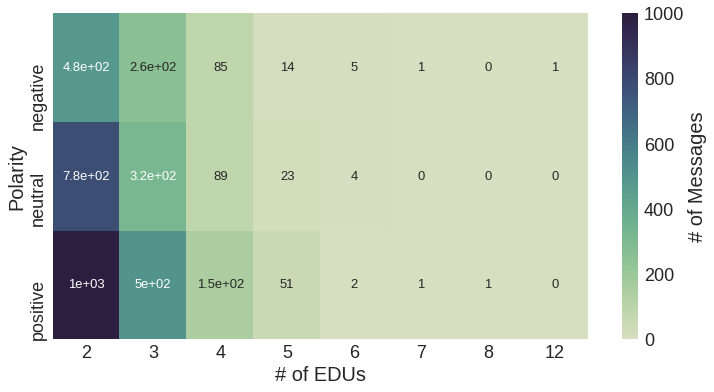
\includegraphics[width=\linewidth]{img/dasa_potts_edu_distribution.png}
      \caption{PotTS}\label{dasa:fig:data-distribution-potts}
    \end{subfigure}
  }
  \centering
  {
    \centering
    \begin{subfigure}{0.7\textwidth}
      \centering
      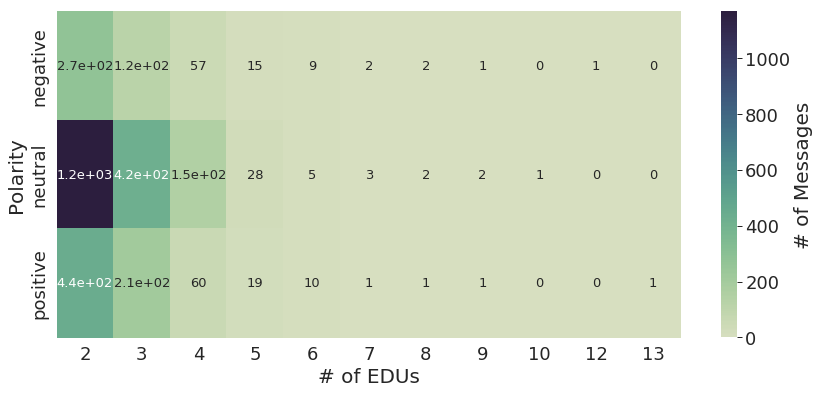
\includegraphics[width=\linewidth]{img/dasa_sb10k_edu_distribution.png}
      \caption{SB10k}\label{dasa:fig:data-distribution-sb10k}
    \end{subfigure}
  }
  \caption[EDU distribution in PotTS and SB10k]{Distribution of
    Elementary Discourse Units and Polarity Classes in the Training and
    Development Sets of PotTS and
    SB10k}\label{dasa:fig:data-distribution}
\end{figure*}

Figure~\ref{dasa:fig:data-distribution} shows the distribution of
elementary discourse units and polarity classes in the training and
development data of both datasets.  As we can see from the graphics,
most of the tweets in both corpora typically have two or three
segments, while messages with more than five EDUs are extremely rare
and rather represent exceptions, which is also not surprising
regarding the maximum length restriction of 140 characters.
Nonetheless, even with this limitation, there still are a few
microblogs with 12 and 13 discourse units.  Since it was somewhat
unusual to see that many segments in a single message, we decided to
look at these tweets in more detail.  As it turned out, such high
number of EDUs typically arose from spurious punctuation marks, which
were carelessly used in texted messages but evidently confused our
segmenter, which had been trained on standard-language data (see
Example~\ref{dasa:exmp:many-segments}).

\begin{example}[SB10k Tweet with 13 EDUs]\label{dasa:exmp:many-segments}
  \noindent\textup{\bfseries\textcolor{darkred}{Tweet:}} { \upshape
    [Guinness on Wheelchairs :]$_1$ [Das .]$_2$ [Ist .]$_3$ [Verdammt
      .]$_4$ [Noch .]$_5$ [Mal .]$_6$ [Einer .]$_7$ [Der .]$_8$
    [Besten .]$_9$ [Werbespots .]$_{10}$ [Des .]$_{11}$ [Jahrzehnts
      .]$_{12}$ [( Auch ...]$_{13}$ }\\
    {\textup{[}Guinness on
      Wheelchairs :\textup{]$_1$} \textup{[}This .\textup{]$_2$}
    \textup{[}Is .\textup{]$_3$} \textup{[}Gosh .\textup{]$_4$}
    \textup{[}Darn .\textup{]$_5$} \textup{[}It .\textup{]$_6$}
    \textup{[}One .\textup{]$_7$} \textup{[}Of .\textup{]$_8$}
    \textup{[}The best .\textup{]$_9$} \textup{[}Commercials
      .\textup{]$_{10}$} \textup{[}Of .\textup{]$_{11}$} \textup{[}The
      Decade .\textup{]$_{12}$} \textup{[}( Also ...\textup{]$_{13}$}}
\end{example}

Another noticeable trend which we also can observe in the data is that
the distribution of the polarity classes in messages with multiple
EDUs largely corresponds to the frequencies of these semantic
orientations in the complete datasets: For example, the positive class
still dominates the PotTS corpus, whereas the neutral polarity
constitues the vast majority of the SB10k set.  Similarly, negative
microblogs again are the least represented group in both cases and
account for 22\% of the former data and 16\% of the latter tweebank.

To obtain RST trees for the segmented messages, we retrained the DPLP
discourse parser of~\citet{Ji:14} on the Potsdam Commentary Corpus
\cite[PCC~2.0; ][]{Stede:14}, after converting all discourse relations
of this dataset to the binary scheme $\{$\textsc{Contrastive},
\textsc{Non-Contrastive}$\}$, as suggested
by~\citet{Bhatia:15}.\footnote{See Table~\ref{dasa:tbl:rst-rels} for
  more details regarding this mapping.}  In contrast to the original
DPLP implementation though, we did not use Brown clusters as features
\cite{Brown:92}, since this resource was not available for German, and
we did not utilize the linear projection of feature values, because
the released parser code did not include this component either.  In
part due to these modifications, but mostly because of the specifics
of the German language, the results of our retrained model were also
considerably lower than the figures reported for the English RST
Treebank~\cite{Carlson:01a}: 0.777, 0.512, and 0.396~\F{} for the
span, nuclearity, and relation prediction on PCC~2.0 versus 82.08,
71.13, and 61.63~\F{} on the English corpus.\footnote{Following
  \citet{Ji:14}, we use the span-based evaluation metric
  of~\citet{Marcu:00}.}

Figure~\ref{dasa:fig:twitter-rst-tree} shows an example of an
automatically induced RST tree.  As we can see, the adapted parser can
correctly distinguish between contrastive and non-contrastive links,
but apparently struggles with the disambiguation of the nuclearity
status, assigning the highest significance to the initial discource
segment (``Mooooiiinn.''  [\emph{Hellloooo!}]), which is merely a
greeting, and weighing the second EDU (``Gegen solche N\"achte hilft
die beste Kur nicht.''  [\emph{Even the best cure won't help against
    such nights.}]) less than the third one (``Aber Kaffee!''
[\emph{But coffee!}]), although traditional RST would consider both
units as equally important and use the multi-nuclear \textsc{Contrast}
relation for them.

\begin{figure*}[htbp!]
  {
\centering
\dirrel{}
        {\rstsegment{\refr{1}}}
        {\textsc{Non-Contrastive}}
        {
        \dirrel{\textsc{Contrastive}}
                {\rstsegment{\refr{2}}}
                {}
                {\rstsegment{\refr{3}}}}

\begin{flushleft}
\begin{rhetoricaltext}
\unit[1]{Mooooiiinn.}
\unit[2]{Gegen solche N\"achte hilft die beste Kur nicht.}
\unit[3]{Aber Kaffee!}
\rstsource{\cite[PotTS; ][]{Sidarenka:16}}
\end{rhetoricaltext}
\end{flushleft}
\caption[Automatic RST tree for a tweet]{Example of an automatically constructed RST-Tree for a Twitter message}\label{dasa:fig:twitter-rst-tree}
}

\end{figure*}

Regarding the distribution of the two coarse-grained discourse
relations, as we can see from
Figure~\ref{dasa:fig:relation-distribution}, the
\textsc{Non-Contrastive} ties clearly dominate both corpora,
accounting for 98\% of all discourse links in PotTS and SB10k.  By
comparison, the precentage of these relations in PCC~2.0 amounts to
90\% and also represents the prevailing majority of all semantic ties
in this dataset.

\begin{figure*}
  \centering
  {
    \centering
    \begin{subfigure}{0.7\textwidth}
      \centering
      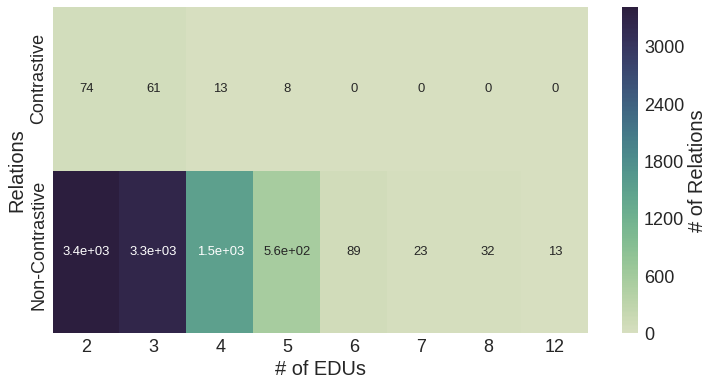
\includegraphics[width=\linewidth]{img/dasa_potts_rel_distribution.png}
      \caption{PotTS}\label{dasa:fig:relation-distribution-potts}
    \end{subfigure}
  }
  \centering
  {
    \centering
    \begin{subfigure}{0.7\textwidth}
      \centering
      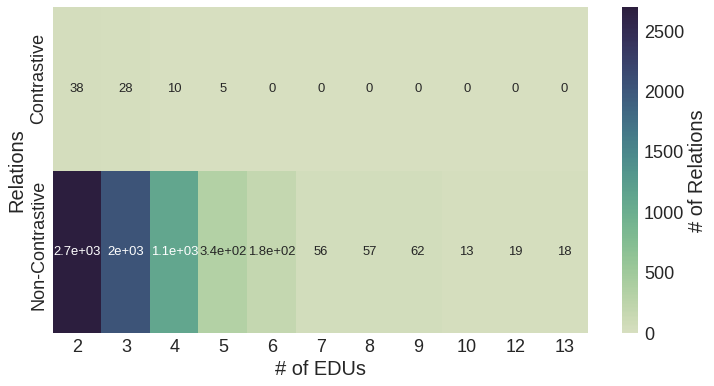
\includegraphics[width=\linewidth]{img/dasa_sb10k_rel_distribution.png}
      \caption{SB10k}\label{dasa:fig:relation-distribution-sb10k}
    \end{subfigure}
  }
  \caption[Relation distribution in PotTS and SB10k]{Distribution of
    Discourse Relations in the Training and Development Sets of PotTS
    and SB10k}\label{dasa:fig:relation-distribution}
\end{figure*}

\section{Discourse-Aware Sentiment Analysis}\label{sec:dasa:data}

% \done[inline]{\citet{Bickerstaffe:10}}

% \citet{Bickerstaffe:10} also considered the rating prediction task,
% addressing this problem with the minimum-spanning-tree (MST) SVM
% approach.  In the initial step of this method, they constructed a
% strongly connected graph whose vertices were associated with the most
% representative example (determined via the average all-pairs Tanimoto
% coefficient) of each star rating and the edge weights represented the
% Tanimoto distances between those nodes.  Afterwards, they determined
% the MST of this graph using the Kruskal's
% algorithm~\cite[see][pp.~567--574]{Cormen:09} and, finally,
% constructed a decision tree from this MST, replacing the MST vertices
% with binary SVM classifiers, which had to discern the respective
% rating groups. An evaluation on the four-star review corpus
% of~\citet{Pang:05} showed an improvement by up to~7\% over the
% previous state of the art, boosting it to 59.37\% average accuracy.

Now, with these prepared data at hand, we are all set to check whether
incorporating the additional discourse information into our
lexicon-based attention system would improve the quality of its
analysis.  However, before we proceed with this check, let us first
make a short digression and revise the most prominent related
approaches to discourse-aware sentiment classification that have been
introduced in the literature so far.

As it turns out, even the very first works on opinion mining already
pointed out the importance of discourse phenomena for determining the
overall polarity of a text.  For example, in the seminal paper
of~\citet{Pang:02}, where the authors tried to predict the semantic
orientation of movie reviews (whether these reviews were thumbs down
or thumbs up), they quickly noticed the fact that it was insufficient
to rely on the mere presence or majority of polarity clues because
these clues could any time be invalidated by a single counter-argument
(see Example~\ref{disc-snt:exmp-pang02}).
\begin{example}[Polarity reversal via discourse antithesis]\label{disc-snt:exmp-pang02}
  \noindent\upshape This film should be brilliant.  It sounds like a
  great plot, the actors are first grade, and the supporting cast is
  good as well, and Stallone is attempting to deliver a good
  performance.  However, it can't hold up. \cite{Pang:02}
\end{example}
\noindent \citet{Polanyi:06} also confirmed the important role of the
text structure, considering discourse connectors and relations as one
of the most significant context factors, which could notably affect
the intensity and polarity of opinionated words.  To prove this claim,
they provided several convincing examples, where concessive discourse
links considerably weakened the strength of an opinion, and, vice
versa, elaborations on sentiments notably increased the persuasiveness
of these judgements.

These observations have rapidly motivated the NLP community to add a
discourse-analysis component to document-level sentiment classifiers.
One of the first such systems was presented by~\citet{Pang:04}, who
tried to improve the classification accuracy on the IMDB corpus by
explicitly pointing the sentiment predictor only to the sentences
which another (discourse-aware) classifier has previously considered
as subjective.  To achieve this goal (\ie{} to distinguish between
subjective and objective statements), \citet{Pang:04} represented the
text as a graph whose vertices corresponded to sentences with their
automatically induced subjectivity scores (which were at first
assigned independently of other clauses) and connected these vertices
via affinity efges to their immediate neighbors.  After adding two
additional abstract nodes representing the subjective and objective
classes, the authors determined the minimum cut of that graph using
the Blum algorithm \cite{Blum:01} and partitioned it into two clusters
(subjective and objective) on that cut.

Although an obvious oversimplification, the core idea that locally
adjacent sentences had to share the same subjective properties (local
coherence) has been dominating the following discourse-aware sentiment
research for almost a decade.  For example, \citet{Riloff:03} also
improved the accuracy of their Na{\"i}ve Bayes predictor of subjective
expressions by $\approx2\%$ after adding a set of discourse-related
features indicating the relative length of the sentence w.r.t. its
neighbors, the average number of subjective clues in the preceding,
current, and following clauses, and the relative number of these clues
with respect to the corresponding sentence lengths.  Similarly,
\citet{Hu:04} achieved better scores on disambiguating users'
polarities towards particular product features after taking the
information about the semantic orientation of previous sentences into
account.

Another important line of DASA research concentrated more on the joint
analysis of opinions, where, in addition to classifying each sentiment
in isolation, the authors also sought to maximize the ``total
happiness'' (or global coherence) of these assignments by ensuring
that similar or related judgements receieved the same or at least
agreeing polarity scores (\citet{Pang:04} also tried to achieve this
objective by constructing and partitioning the text graph).  One of
the most notable works in this direction was done by
\citet{Snyder:07}, who introduced the Good Grief algorithm for
predicting users' satisfaction with different restaurant aspects.
Another important contribution was made by
\citet{Somasundaran:08a,Somasundaran:08}, who proposed the concept of
\emph{opinion frames} (OF)---a special data structure for representing
the relations between the opinions in discourse.  Depending on the
type of these opinions (whether arguing~[\emph{A}] or
sentiment~[\emph{S}]), their polarity towards the target (whether
positive~[\emph{P}] or negative~[\emph{N}]), and semantic relationship
between the two targets (whether alternative~[\emph{Alt}] or the
same~[\emph{same}]), the authors distinguished 32 types of possible
frames: \emph{SPSPsame}, \emph{SPSNsame}, \emph{APAPalt}, etc.,
dividing them into reinforcing and non-reinforcing ones.  Later on,
\citet{Somasundaran:09a,Somasundaran:09b} also presented two joint
inference frameworks (one of which was based on the iterative
classification algorithm and another one used the integer linear
programming) for determining the best configuration of single opinions
and their respective connecting frames, achieving 77.72\% accuracy of
frame prediction on the AMI meeting corpus~\cite{Carletta:05}, when
given oracle information about the opinions.

%% \done[inline]{\citet{Somasundaran:09a,Somasundaran:09b}}

%% In a later work, \citet{Somasundaran:09b,Somasundaran:09a} also
%% introduced a joint inference framework based on the Iterative
%% Classification Algorithm (ICA) and Integer Linear Programming (ILP)
%% for joinly predicting the best configuration of single opinions and
%% their frames.  In this approach, the authors first applied a local SVM
%% classifier to compute the probabilities of polarity classes (positive,
%% negative, or neutral) of individual dialog acts and then harnessed the
%% ICA and ILP systems to determine which of the predicted opinions were
%% connected via opinion frames and whether these frames were reinforcing
%% or not.  Given a perfect information about the opinion links, this
%% joint method outperformed the local classifier by more than 9
%% percentage points, reaching 77.72\% accuracy on the AMI meeting
%% corpus~\cite{Carletta:05}.

%% \done[inline]{\citet{Mao:06}}

%% \citet{Mao:06} proposed the idea of isotonic CRFs in which they
%% explicitly modeled the constraint that features which were stronger
%% associated with either polarity classes had to have higher
%% coefficients than less predictive attributes.  After proving that this
%% formalism also allowed to directly model the ordinal scale of
%% sentiment scores (with lower CRF outputs indicating the negativity of
%% a sentence, and higher scores showing its positive class), the authors
%% used this approach to model the sentiment flow in a document.  For
%% this purpose, they first predicted the polarity value for each
%% sentence of a document in isolation and then convolved these outputs
%% with a Gaussian kernel, getting a smoothed polarity curve for the
%% whole analyzed text at the end.
%% \done[inline]{\citet{Thomas:06}}

%% \citet{Thomas:06} enhanced an SVM-based sentiment classification
%% system for predicting speaker's attitude in political speeches with
%% information about the inter-speaker agreement, incorporating these
%% links into the global cost function.  Thanks to this change, the
%% authors achieved $\approx$4\% improvement in accuracy (from 66.05 to
%% 70.81\%) over the baseline classifer which analyzed each utterance in
%% isolation.

An attemt to reunite local and global coherence again was made by
\citet{McDonald:07}, who proposed a joint framework based on
\emph{latent variables} for simultaneously predicting the polarity of
a document and its constituent parts (which could be either paragraphs
or sentences).  For this purpose, the authors considered the semantic
orientation of the whole text and its single sentences as unobserved
variables in a Markov random field, connecting each such sentence node
to the vertices of its adjacent clauses and the overal polarity node
of the complete document, and then figuring out the best configuration
of all variables at the end.  A similar approach was also suggested
by~\citet{Sadamitsu:08}, who attained 82.74\% accuracy on predicting
the polarity of customer reviews with the help of hidden conditional
random fields.

Another latent-variable approach was presented by
\citet{Yessenalina:10}, who tried to predict the overall semantic
orientation of a document by first selecting a subset of the most
indicative sentences and then classifying the document (as either
positive or negative) with the help of this selection.  To achieve
this goal, the authors adopted the latent-SVM method of \citet{Yu:09}
by first training a linear classifier on individual sentences with
latent classes and then making the final prediction using 30\% of
those clauses which the classifier was most sure about.  With this
method, \citet{Yessenalina:10} could attain 93.22\% accuracy on the
movie review corpus of \citet{Pang:04} and reach 77.09\% on a
collection of congressional floor debates \cite{Thomas:06}.

A common drawback of all of the above approaches though is their
complete ignoring of traditional discourse theories and, as a
consequence of this, too coarse approximation of discourse structure
(which essentially boils down to either connecting nearby sentences,
or creating a densely connected graph).  Among the first who tried to
overcome this omission were \citet{Voll:07}, who came up with two
different ways of making their lexicon-based sentiment calculator
\cite[SO-CAL; ][]{Taboada:11} aware of discourse information: In the
first method, they let the classifier analyze only those discourse
segments which appeared in the top-post nuclei of the sentences (using
automatically derived RST trees for determining such EDUs).  In the
second attempt, they restricted SO-CAL's input only to the clauses
which had been previously classified as pertaining to the main topic
of the text.  Unfortunately, the RST-based solution did not work out
as well as expected and failed to outperform even the
discourse-unaware baseline, yielding only 69\% precision on a corpus
of Epinion reviews \cite{Taboada:06}.  This mishap, however, might be
partially due to the fact that the authors completely ignored all
nuclei and satellites apart from the roots and also disregarded all
inter-sentential relations.  The second alternative, however, turned
out to work fairly well, achieving 73\% accuracy on this two-class
prediction task.

Other ways of incorporating discourse information into a sentiment
system were explored by \citet{Heerschop:11}, who experimented with
three different approaches:
\begin{inparaenum}[(i)]
\item increasing the polarity scores of words which appeared near
  the end of the document,
\item assigning higher weights to tokens in the nuclei of RST trees
  rather than satellites, and, finally,
\item training a genetic algorithm, which learned separate scores for
  the nuclei and eight types of satellite nodes (\textsc{Attribution},
  \textsc{Background}, \textsc{Cause}, etc.).
\end{inparaenum}
An evaluation of these methods on the movie review corpus
of~\citet{Pang:04} showed superior performance of the first option
(0.608 accuracy and 0,597 macro\F).  The authors, however, could
significantly improve the results of the last classifier at the end,
after adding an offset to the decision boundary, which increased both
its accuracy and macro~\F-measure to 0.72.

Other notable works on RST-based sentiment prediction were done by
\citet{Zhou:11}, who used a set of heuristic rules to infer possible
polarity shifts of discourse units based on their nuclearity status
and links to the parent units, which allowed them to attain a
statistically significant improvement in sentence-level polarity
classification on the NTCIR MOAT corpus~\cite{Xu:10}; \citet{Zirn:11},
who applied a lexicon-based sentiment system to compute the polarity
scores of elementary discourse units, and then enforced the
consistency of these assignments over an automatically derived RST
tree with the help of of Markov logic contraints; and \citet{Wang:13},
who also first computed polarity scores of isolated discourse units
and then estimated the polarity of the whole document by taking a
linear combination of these EDU scores, multiplying them with
automatically learned coefficients.\footnote{Similarly to the approach
  of~\citet{Zirn:11}, these coefficients depended on the status of the
  segment in the RST tree (whether nucleus or sattelite) and relation,
  which connected the respective discourse node to the ancestor.}  A
similar system was also described by \citet{Chenlo:13,Chenlo:14}, who
used their model to analyze user blog posts, achieving significantly
better results on the TREC corpus \cite{Macdonald:09} than any
discourse-unaware baselines.

Among the most recent advances in RST-based opinion mining, we should
especially emphasize the work of \citet{Bhatia:15}, who proposed two
different sentiment analysis systems:
\begin{itemize}
\item discourse depth reweighting (DDR)
\item and rhetorical recursive neural network (R2N2).
\end{itemize}
In the former approach, they estimated the relevance $\lambda_i$ of
each elementary discourse unit $i$ as:
\begin{equation*}
  \lambda_i = \max\left(0.5, 1 - d_i/6\right),
\end{equation*}
where $d_i$ stands for the depth of the $i$-th EDU in the document's
discourse tree; and computed the sentiment score $\sigma_i$ of that
unit as the dot product of its binary feature vector $\mathbf{w}_i$
(token unigrams) with the coefficients of these features $\theta$
(polarity scores of the respective unigrams):
\begin{equation*}
  \sigma_i = \theta^{\top}\cdot\mathbf{w}_i,
\end{equation*}
Afterwards, the authors calculated the overall polarity of the
document~$\Psi$ as the sum of the predicted sentiment scores for all
units, multiplying these weights by the importance factors~$\lambda$:
\begin{equation*}
  \Psi = \sum_i\lambda_i\mathbf{\theta}^T\cdot\mathbf{w}_i = \mathbf{\theta}^T\cdot\sum_i\lambda_i\mathbf{w}_i,
\end{equation*}

In the R2N2 method, \citet{Bhatia:15} adopted the RNN approach
of~\citet{Socher:13} by recursively computing the polarity score of
each discourse unit $i$ as:
\begin{equation*}
  \psi_i = tanh\left(K_n^{(r_i)} \psi_{n(i)} + K_s^{(r_i)}\psi_{s(i)} \right),
\end{equation*}
where $K_n^{(r_i)}$ and $K_s^{(r_i)}$ denote the nucleus and satellite
coefficients associated with the rhetorical relation $r_i$, whereas
$\psi_{n(i)}$ and $\psi_{s(i)}$ represent the sentiment scores of the
nucleus and satellite nodes of the $i$-th discourse node.  This system
achieved formidable 84.1\% prediction accuracy on the two-class moview
review corpus of~\citet{Pang:04} and reached 85.6\% on the dataset
of~\citet{Socher:13}.

For the sake of completeness, we should note that there also exist
discourse-aware sentiment approaches which build upon the PDTB and
SDRT frameworks: For example, \citet{Trivedi:13} presented a method
based on the latent structural SVM \cite{Yu:09}, in which they
represented each sentence as a set of features associated with the
potential polarity of that document $y\in\{-1, +1\}$ and subjectivity
class of the sentence $h_i \in \{0, 1\}$ produced by the function
$\mathbf{f}(y, \mathbf{x}_i, h_i)$, where $\mathbf{x}_i$ was the
surface form of the $i$-th sentence from which the features were
extracted.  One such attribute could, for example, be \texttt{<+1,
  ``love'', 1>}, which would indicate the token ``love'' in a
subjective sentence of a positive document. Since the true assignment
of the variables $h_i$ was unknown though, the authors regarded this
value as a latent variable and tried to predict the most likely
semantic orientation of document $\hat{y}$ by inferring the most
probable assignment of $h$:
\begin{equation*}
  \hat{y} = \argmax_y\left(\max_{\mathbf{h}}\mathbf{f}(y, \mathbf{x},
  \mathbf{h})\mathbf{w}^{\top}\right).
\end{equation*}
To ensure that this assignment was coherent over the text, the authors
enhanced their original feature function with an additional set of
\emph{transitional} attributes, which indicated whether two adjacent
sentences were likely to share the same subjectivity given the
discourse connector of the second clause.  With the help of these
features, were able to boost the prediction accuracy on the movie
review corpus of~\citet{Maas:11} from 88.21 to 91.36\% in comparison
with the connector-unaware model.

The first steps towards an SDRT-inspired approach were made by
\citet{Asher:08}, who presented an annotation scheme and pilot corpus
of English and French texts labeled with their discourse structure
according to the SDRT theory and augmented with an additional
sentiment layer.  To this end, the authors asked the annotators to
ascribe one of the four opinion categories (reporting, judgement,
advice, or sentiment) along with their subcategories (e.g., inform,
assert, blame, recommend) to each discourse unit which featured at
least one opinionated word from a sentiment lexicon.  Afterwards, they
showed that with a simple set of rules, one could easily propagate
opinions through the discourse graphs, increasing their strengths or
reversing their polarity, depending on the type of discourse relations
that connected the segments.

In general, however, PDTB- and SDRT-based sentiment analysis methods
are much less common than RST-inspired techniques, and since the focus
of this chapter is mainly on RST, we will next present an evaluation
of the most common approaches from this paradigm on the PotTS and
SB10k data.  To this end, we have reimplemented the DDR and R2N2
systems of~\citet{Bhatia:15}

\begin{table}[h]
  \begin{center}
    \bgroup \setlength\tabcolsep{0.1\tabcolsep}\scriptsize
    \begin{tabular}{p{0.162\columnwidth} % first columm
        *{9}{>{\centering\arraybackslash}p{0.074\columnwidth}} % next nine columns
        *{2}{>{\centering\arraybackslash}p{0.068\columnwidth}}} % last two columns
      \toprule
      \multirow{2}*{\bfseries Method} & %
      \multicolumn{3}{c}{\bfseries Positive} & %
      \multicolumn{3}{c}{\bfseries Negative} & %
      \multicolumn{3}{c}{\bfseries Neutral} & %
      \multirow{2}{0.068\columnwidth}{\bfseries\centering Macro\newline \F{}} & %
      \multirow{2}{0.068\columnwidth}{\bfseries\centering Micro\newline \F{}}\\
      \cmidrule(lr){2-4}\cmidrule(lr){5-7}\cmidrule(lr){8-10}

      & Precision & Recall & \F{} & %
      Precision & Recall & \F{} & %
      Precision & Recall & \F{} & & \\\midrule

      \multicolumn{12}{c}{\cellcolor{cellcolor}PotTS}\\

      %% General Statistics:
      ZRN &  &  &  & %
      &  &  & %
      &  &  & %
      & \\

      %% General Statistics:
      DDR & 0.73 & 0.77 & 0.75 & %
      0.54 & 0.59 & 0.56 & %
      0.69 & 0.61 & 0.65 & %
      0.655 & 0.674\\

      %% General Statistics:
      R2N2 &  &  &  & %
      &  &  & %
      &  &  & %
      & \\

      %% General Statistics:
      \textsc{Last} & 0.52 & 0.83 & 0.64 & %
      0.57 & 0.17 & 0.26 & %
      0.61 & 0.43 & 0.5 & %
      0.453 & 0.549\\

      %% General Statistics:
      \textsc{Root} & 0.56 & 0.73 & 0.64 & %
      0.58 & 0.22 & 0.32 & %
      0.55 & 0.54 & 0.54 & %
      0.481 & 0.56\\

      %% General Statistics:
      \textsc{No-Discourse} & 0.73 & 0.82 & 0.77 & %
      0.61 & 0.56 & 0.58 & %
      0.72 & 0.66 & 0.69 & %
      0.677 & 0.706\\

      \multicolumn{12}{c}{\cellcolor{cellcolor}SB10k}\\

      %% General Statistics:
      ZRN &  &  &  & %
      &  &  & %
      &  &  & %
      & \\

      %% General Statistics:
      DDR & 0.59 & 0.63 & 0.61 & %
      0.48 & 0.44 & 0.46 & %
      0.77 & 0.76 & 0.77 & %
      0.534 & 0.681\\

      %% General Statistics:
      R2N2 &  &  &  & %
      &  &  & %
      &  &  & %
      & \\

      %% General Statistics:
      \textsc{Last} & 0.56 & 0.55 & 0.56 & %
      0.46 & 0.29 & 0.36 & %
      0.73 & 0.8 & 0.76 & %
      0.459 & 0.661\\

      %% General Statistics:
      \textsc{Root} & 0.51 & 0.55 & 0.53 & %
      0.4 & 0.3 & 0.35 & %
      0.74 & 0.76 & 0.75 & %
      0.438 & 0.64\\

      %% General Statistics:
      \textsc{No-Discourse} & 0.64 & 0.69 & 0.66 & %
      0.45 & 0.45 & 0.45 & %
      0.82 & 0.79 & 0.8 & %
      0.557 & 0.713\\\bottomrule
    \end{tabular}
    \egroup
    \caption[Evaluation of DASA methods]{Evaluation of discourse-aware
      sentiment analysis methods\\ {\small
        ZRN~--~\citet{Zirn:11},
        WNG~-~\citet{Wang:13},
        BHT~--~\citet{Bhatia:15},
        \textsc{Last}~--~polarity determined by the last EDU,
        \textsc{Last}~--~polarity determined by the root nucleus,
        \textsc{No-Discourse}~--~discourse-unaware lexicon-based
        attention model with one Bi-LSTM layer}}
    \label{dasa:tbl:res}
  \end{center}
\end{table}

\section{Evaluation}

\subsection{Relation Scheme}

\begin{table}[h]
  \begin{center}
    \bgroup \setlength\tabcolsep{0.1\tabcolsep}\scriptsize
    \begin{tabular}{p{0.17\columnwidth} % first columm
        *{1}{>{\centering\arraybackslash}p{0.4\columnwidth}}
        *{1}{>{}p{0.4\columnwidth}}} % next two columns
      \toprule
      \textbf{Scheme} & \textbf{Relation Set} & \textbf{Equivalence Classes}\\\midrule

      \textsc{PCC} & \{ \textsc{Antithesis}, \textsc{Background},
      \textsc{Cause}, \textsc{Circumstance}, \textsc{Concession},
      \textsc{Condition}, \textsc{Conjunction}, \textsc{Contrast},
      \textsc{Disjunction}, \textsc{E-Elaboration},
      \textsc{Elaboration}, \textsc{Enablement},
      \textsc{Evaluation-N}, \textsc{Evaluation-S}, \textsc{Evidence},
      \textsc{Interpretation}, \textsc{Joint}, \textsc{Justify},
      \textsc{List}, \textsc{Means}, \textsc{Motivation},
      \textsc{Otherwise}, \textsc{Preparation}, \textsc{Purpose},
      \textsc{Reason}, \textsc{Restatement}, \textsc{Restatement-MN},
      \textsc{Result}, \textsc{Sequence}, \textsc{Solutionhood},
      \textsc{Summary}, \textsc{Unconditional}, \textsc{Unless},
      \textsc{Unstated-Relation}\} & \\

      \citet{Heerschop:11} & \{\textsc{Attribution},
      \textsc{Background}, \textsc{Cause}, \textsc{Condition},
      \textsc{Contrast}, \textsc{Elaboration}, \textsc{Enablement},
      \textsc{Explanation}, \textsc{\bfseries Other}\} & \\

      \citet{Zhou:11} & \{\textsc{Contrast}, \textsc{Condition},
      \textsc{Continuation}, \textsc{Cause}, \textsc{Purpose},
      \textsc{\bfseries Other}\} & \textsc{Contrast} $\defeq$
      \{\textsc{Antithesis}, \textsc{Concession}, \textsc{Otherwise},
      \textsc{Contrast}\};\newline \textsc{Continuation} $\defeq$
      \{\textsc{Continuation}, \textsc{Parallel}\};\newline
      \textsc{Cause} $\defeq$ \{\textsc{Evidence}, \textsc{Volitional
        Cause}, \textsc{Nonvolitional-Cause},
      \textsc{Volitional-Result}, \textsc{Nonvolitional-Result}\};\\

      \citet{Chenlo:13} & \{\textsc{Attribution}, \textsc{Background},
      \textsc{Cause}, \textsc{Comparison}, \textsc{Condition},
      \textsc{Consequence}, \textsc{Contrast}, \textsc{Elaboration},
      \textsc{Enablement}, \textsc{Evaluation}, "Explanation",
      \textsc{Joint}, \textsc{Otherwise}, \textsc{Temporal},
      \textsc{\bfseries Other}\} & \\

      \citet{Bhatia:15} & \{\textsc{Contrastive},
      \textsc{\bfseries Non-Contrastive}\} & \textsc{Contrastive} $\defeq$
      \{\textsc{Antithesis}, \textsc{Antithesis-E},
      \textsc{Comparison}, \textsc{Concession},
      \textsc{Consequence-S}, \textsc{Contrast},
      \textsc{Problem-Solution}\}.\\\bottomrule
\end{tabular}
    \egroup
    \caption[RST relations used in different discourse-aware sentiment
      methods]{RST relations used in the original Potsdam Commentary
      Corpus and different discourse-aware sentiment methods\\ {\small
        (default relation [which subsumes the rest of the links] is
        highlighted in \textbf{boldface})}}
    \label{dasa:tbl:rst-rels}
  \end{center}
\end{table}

\begin{table}[h]
  \begin{center}
    \bgroup \setlength\tabcolsep{0.1\tabcolsep}\scriptsize
    \begin{tabular}{p{0.22\columnwidth} % first columm
        *{3}{>{\centering\arraybackslash}p{0.25\columnwidth}}} \toprule

      \textbf{Relation Scheme} & \textbf{Span \F{}} &
       \textbf{Nuclearity \F{}} & \textbf{Relation \F{}}\\\midrule

      \textsc{PCC} & 0.776 & 0.534 & 0.326\\

      \citet{Heerschop:11} & 0.774 & 0.51 & 0.361\\

      \citet{Zhou:11} & 0.776 & 0.501 & 0.388\\

      \citet{Chenlo:13} & 0.769 & 0.505 & 0.362\\

      \citet{Bhatia:15} & 0.777 & 0.512 & 0.396\\\bottomrule
\end{tabular}
    \egroup
    \caption[Results of RST parser on PCC~2]{Results of automatic RST
      parser on PCC~2.0 with different relation schemes}
    \label{dasa:tbl:rst-rels}
  \end{center}
\end{table}

\section{Summary and Conclusions}
